\documentclass[final]{beamer}
\usepackage{multimedia}
\usepackage{color}
\usepackage[normalem]{ulem}
\usepackage{adjustbox}
\graphicspath{{figures/}}

\newcommand{\comment}[1]{}
\definecolor{grigio}{rgb}{.8, .8, .8}

\mode<beamer>{%
	\usetheme{default}
  \usecolortheme{default}
}
\titlegraphic{
\includegraphics[width=0.3\textwidth]{LogoUPF_CBC}\hspace{0.5cm}
\includegraphics[width=0.3\textwidth]{logo_italian_academy}\hspace{0.5cm}
\includegraphics[width=0.15\textwidth]{columbia}}
\title[Effective connectivity]{\textbf{Whole brain effective connectivity from fMRI data}}
\author{Andrea Insabato}
\date{November 27th, 2017}

\begin{document}


\begin{frame}<handout:0>
  \titlepage
\end{frame}

\begin{frame}
\transdissolve
\frametitle{Whole brain connectivity}
\begin{columns}
\begin{column}{0.5\textwidth}
	\begin{itemize}
		\item Whole brain is divided in ROIs (parcellation)
		\item Average activity in each ROI
		\item Connectivity between ROIs
	\end{itemize}
\end{column}
\begin{column}{0.5\textwidth}
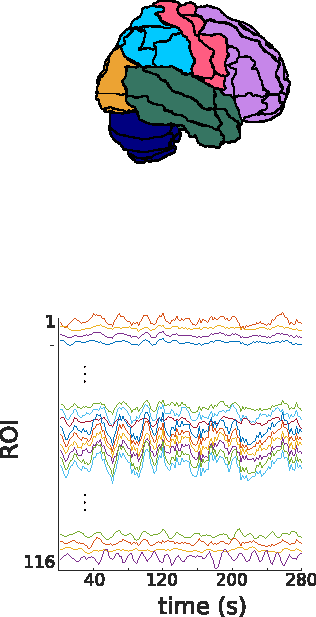
\includegraphics[width=0.5\columnwidth]{parcellation}
\end{column}
\end{columns}
\end{frame}

\begin{frame}
\transdissolve
\frametitle{Functional Connectivity (FC)}
\begin{columns}
\begin{column}{0.5\textwidth}
\includegraphics<1->[width=0.7\columnwidth]{FC}
\end{column}
\begin{column}{0.5\textwidth}
	\begin{itemize}
			\pause
		\item Pearson correlation between ROIs
			\pause
		\item Dense 
			\pause
		\item Symmetric: no directionality of interactions 
	\end{itemize}
\end{column}
\end{columns}
\end{frame}

\begin{frame}
\transdissolve
\frametitle{Effective Connectivity (EC)}
\begin{columns}
\begin{column}{0.5\textwidth}
\includegraphics<1->[width=0.8\columnwidth]{net}
\end{column}
\begin{column}{0.5\textwidth}
	\begin{itemize}
			\pause
		\item Network model 
			\pause
		\item Sparse 
			\pause
		\item Asymmetric: directionality of interactions 
	\end{itemize}
\end{column}
\end{columns}
\end{frame}

\begin{frame}
\transdissolve
\frametitle{Outline}
\begin{itemize}
		\pause
	\item Network model
		\pause
	\item EC based subject and condition identification
		\pause
	\item Estimation of model parameters
\end{itemize}
\end{frame}

\begin{frame}
\transdissolve
\frametitle{Network model}
\begin{itemize}
		\pause
	\item Each node is an Ornstein-Uhlenbeck process 
		\pause
	\item $dx_i(t) = [-\frac{x_i(t)}{\tau_i} + \sum_{j\ne i} C_{ij} x_j + \eta_i]dt + dB_i;\qquad dB_i\sim\mathcal{N}(0,\sigma_i^2)$ 
\end{itemize}
\begin{center}
\includegraphics<1->[width=0.5\columnwidth]{net}
\end{center}
\end{frame}

\begin{frame}
\frametitle{}
\begin{center}
{Estimation of parameters postponed\ldots}
\end{center}
\end{frame}

\begin{frame}
\frametitle<1>{Characterization of whole brain networks underlying ``mental'' states}
\frametitle<2>{Characterization of whole brain networks underlying watching a movie}
\frametitle<3>{Characterization of whole brain networks underlying remembering}
\frametitle<4>{Characterization of whole brain networks underlying calculating}
\frametitle<5>{Characterization of whole brain networks underlying pathological states (dementia, autism, depression, etc.)}
\frametitle<6->{Characterization of whole brain networks underlying ``mental'' states}
\transdissolve
\begin{itemize}
	\item<7-> Separate different sources of varibility
	\visible<9->{
	\begin{itemize}
		\item classify subjects
		\item classify conditions 
		\item extract networks underlying each classification
	\end{itemize}
	}
\end{itemize}
\begin{center}
	\visible<8->{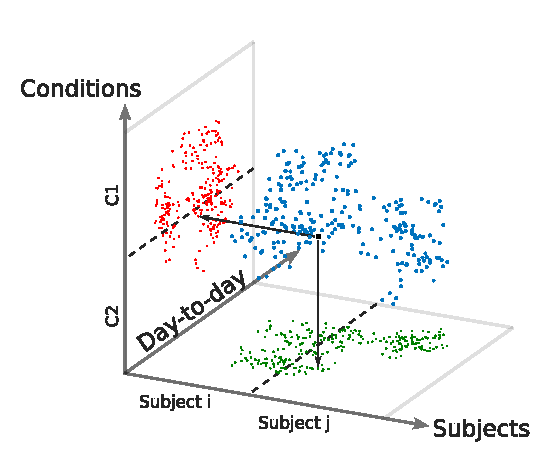
\includegraphics[width=0.5\columnwidth]{subj_cond_idea}}
\end{center}
\end{frame}

\begin{frame}
\transdissolve
\frametitle{Datasets}
	\centering
\adjustbox{max width=\textwidth}{
\begin{table}[t!]
\begin{tabular}{l||l|l|l|l}
Dataset name	& Acquisition	 & Number of subjects	 & Sessions per subject	 & Session duration \\
\hline
\hline
Dataset A1	& Day2day project				 & 6			 & 40-50		 & 5 minutes \\
Dataset B	& CoRR						 & 30			 & 10			 & 10 minutes \\
Dataset C	& Gilson et al. 2017, Mantini et al. 2012	 & 19			 & 3 resting; 2 movie	 & 10 minutes \\
\end{tabular}
\end{table}
}
\end{frame}

\begin{frame}
\transdissolve
\frametitle{Subjects classification}
\begin{itemize}
		\pause
	\item Finn (Nat. Neuro. 2015): FC of $\sim100$ subjects, 5 sessions per subject, Nearest Neighbor, 54-94\% accuracy   
		\pause
	\item Our approach:
		\pause
		\begin{itemize}
	\item Comparison between FC and EC
		\pause
	\item Multinomial logistic regression (interpretability of fitted classifier)
		\pause
	\item \textbf{Test-retest} dataset (10-50 sessions per subject): 
		\pause
		\begin{itemize}
			\item accurate assessment of test accuracy 
		\pause
			\item impact of training set size
		\end{itemize}
		\end{itemize}
\end{itemize}
\end{frame}

\begin{frame}
\transdissolve
\frametitle{Multinomial Logistic Regression (MLR)}
\begin{itemize}
	\item $C_k = softmax(\sum_j^N \beta_{jk} x_j)$
\pause
\item allows to estimate the most relevant features for the classification
	\item Recursive feature elimination: 
		\begin{itemize}
			\item recursively remove feature $i = \operatorname*{arg\,min}_j \sum_k \beta_{jk}$
			\item survival time reflects relevance of each link
		\end{itemize}
\end{itemize}
\end{frame}

\begin{frame}
\frametitle{Subjects classification}
\begin{center}
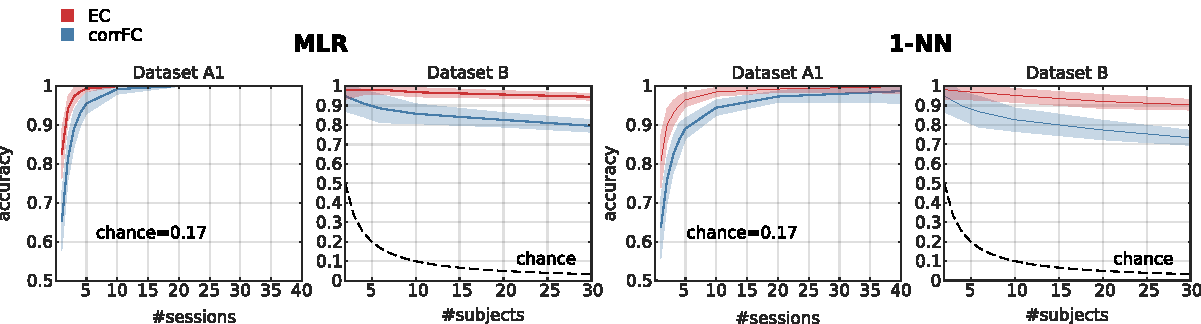
\includegraphics[width=0.95\columnwidth]{class_subj}
\end{center}
\end{frame}

\begin{frame}
\frametitle{Subjects classification}
Classification accuracy using subsets of links according to RFE ranking
\begin{center}
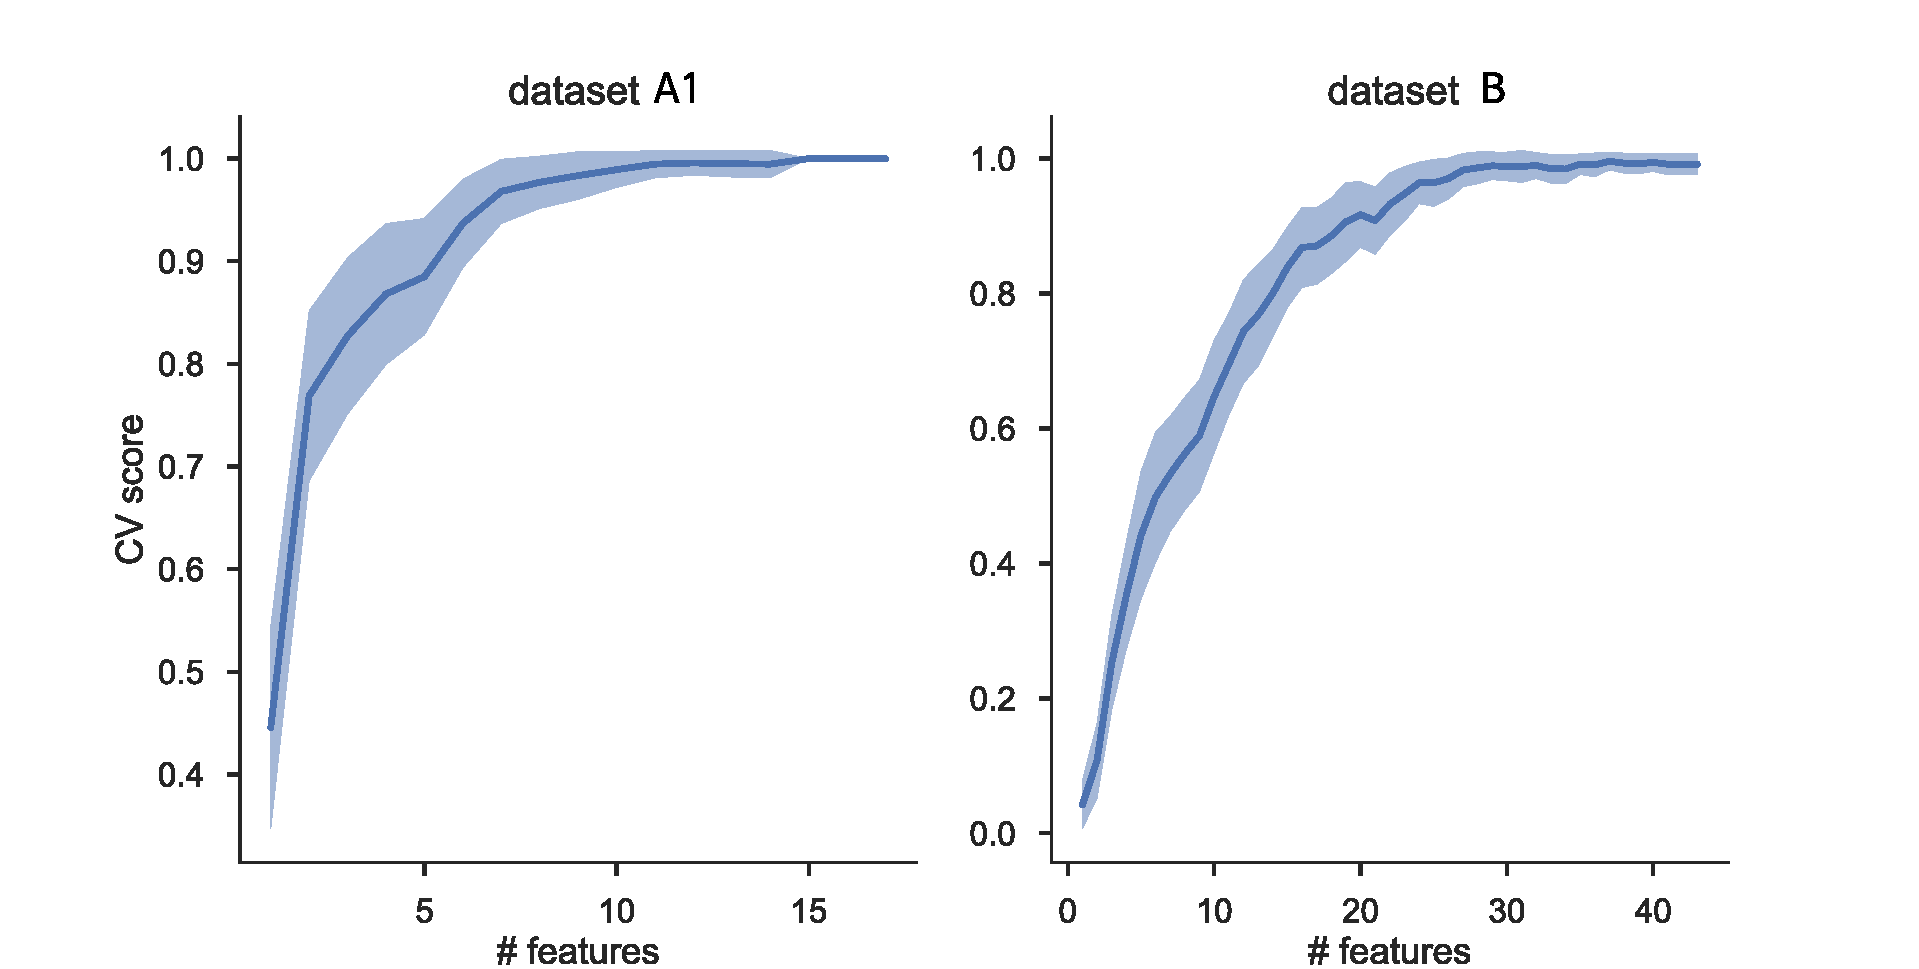
\includegraphics[width=0.8\columnwidth]{subj_varying_links}
\end{center}
\end{frame}

\begin{frame}
\frametitle{Subjects classification}
\begin{center}
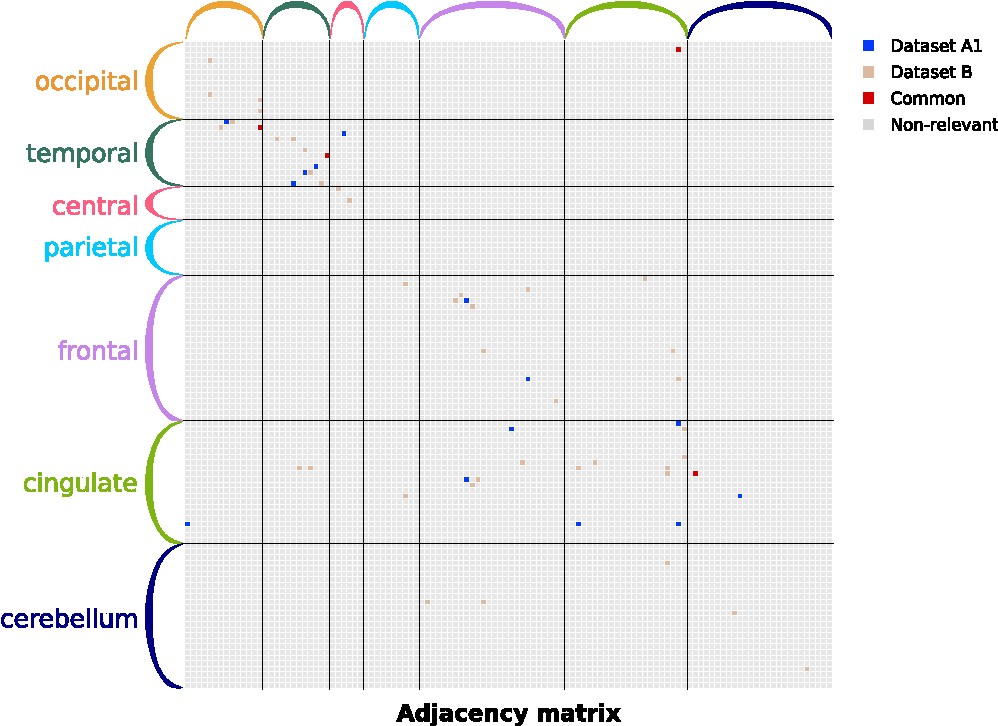
\includegraphics[width=0.9\columnwidth]{subj_net}
\end{center}
\end{frame}

\begin{frame}
\frametitle{Subjects classification}
Average RFE ranking by subsystem
\begin{center}
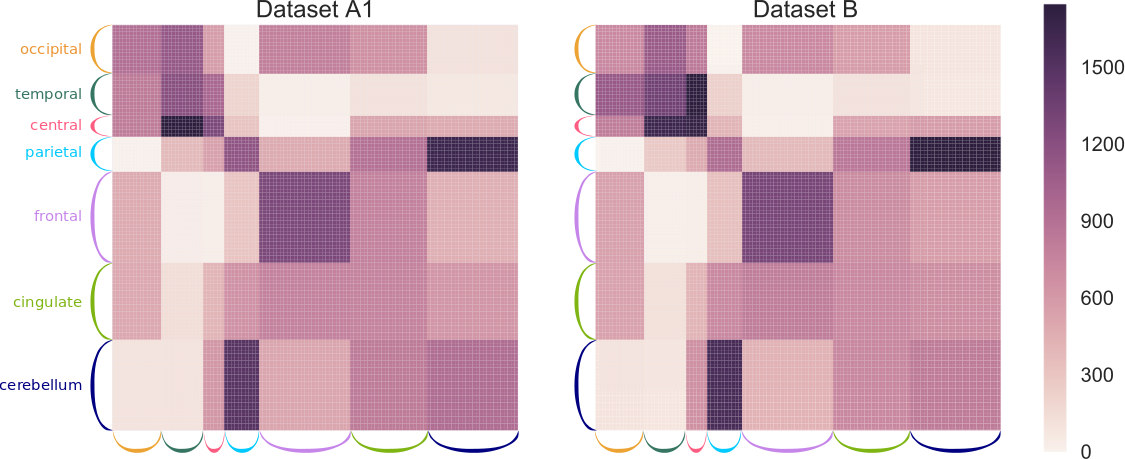
\includegraphics[width=0.9\columnwidth]{avg_ranking_subsystems}
\end{center}
\end{frame}

\begin{frame}
\frametitle{Subjects classification}
Number of overlapping links is much higher than expected by chance
\begin{center}
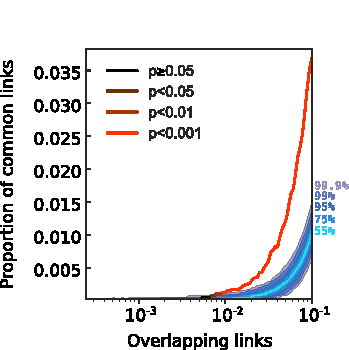
\includegraphics[width=0.5\columnwidth]{subj_H0}
\end{center}
\end{frame}

\begin{frame}
\frametitle{Condition classification}
Dataset C: resting $\Leftrightarrow$ movie viewing\\[0.4cm]
\pause
Classification accuracy using subsets of links according to RFE ranking
\begin{center}
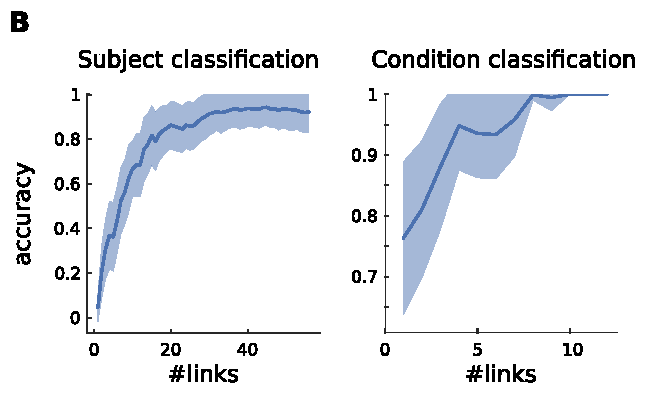
\includegraphics[width=0.8\columnwidth]{subj_cond_results}
\end{center}
\end{frame}

\begin{frame}
\frametitle{Condition classification}
\begin{center}
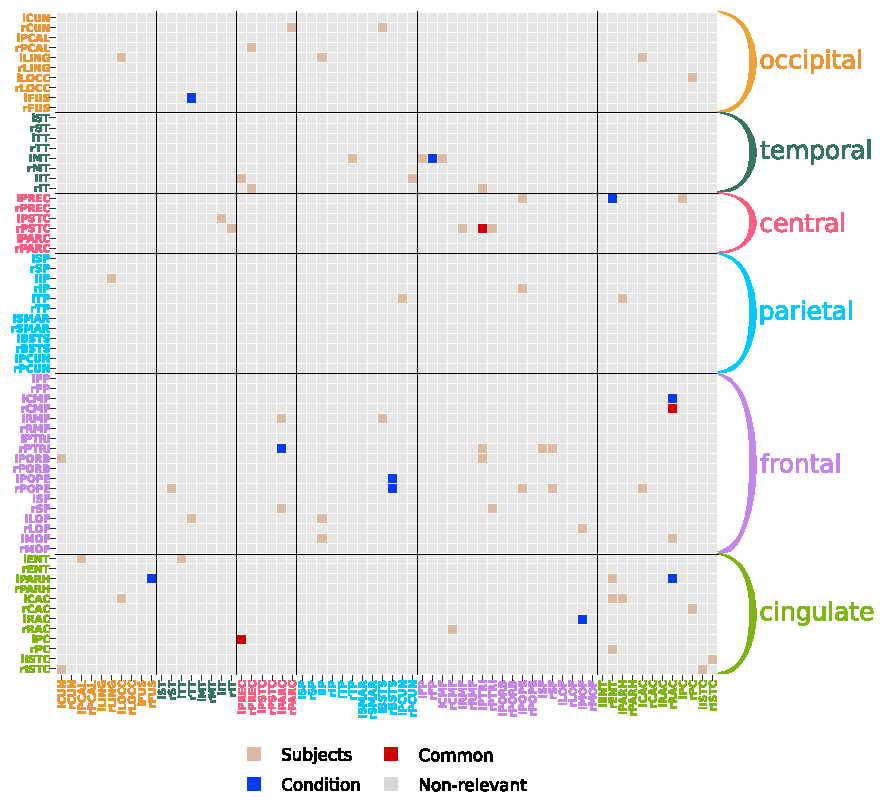
\includegraphics[width=0.65\columnwidth]{subj_cond_matrix}
\end{center}
\end{frame}

\begin{frame}
\frametitle{Condition classification}
Number of overlapping links is similar to that expected by chance
\begin{center}
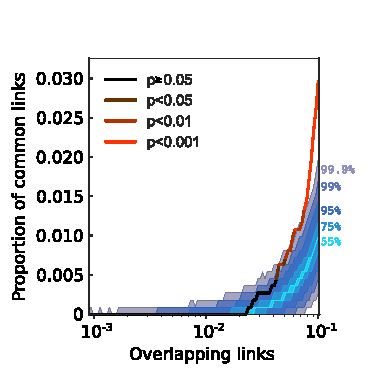
\includegraphics[width=0.5\columnwidth]{cond_H0}
\end{center}
\end{frame}

\begin{frame}
\frametitle{Condition classification}
Subjects and conditions networks
\begin{center}
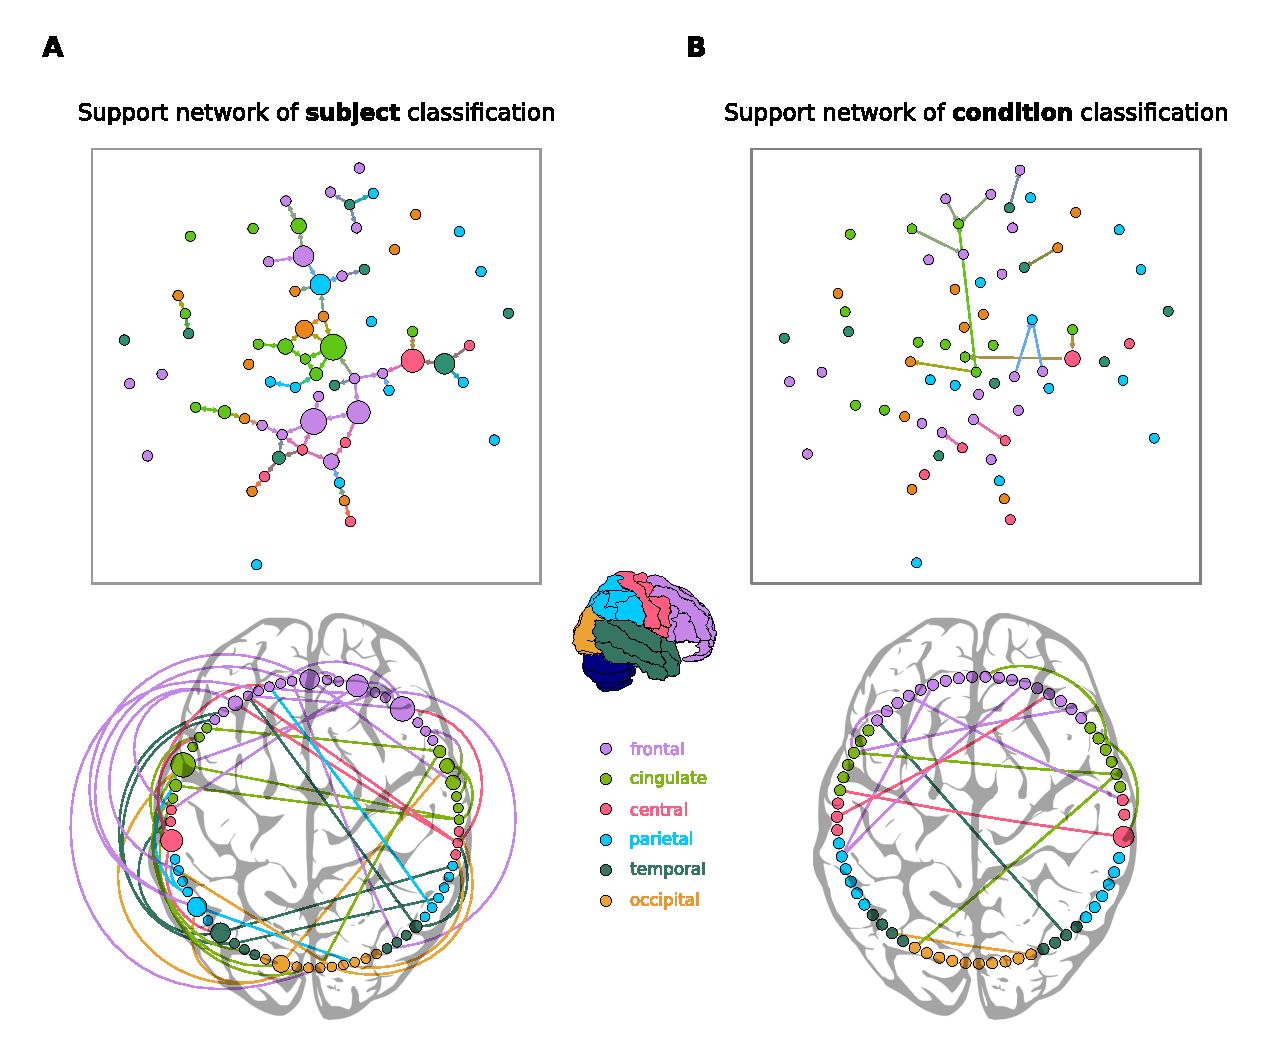
\includegraphics[width=0.7\columnwidth]{fig5}
\end{center}
\end{frame}

\begin{frame}
	\frametitle{Summary (ad interim)}
	\begin{itemize}
		\item MOU model estimates whole brain connectivity
		\item Classification of subjects identity based on estimated connectivity achieves very high accuracy with few recording sessions per subject
		\item Effective connectivity is more reliable than correlation-based functional connectivity
		\item Classification of behavioral conditions and subjects identity on the same dataset achieves very high accuracy
		\item Subjects and condition specific networks show very different properties
	\end{itemize}
\end{frame}

\begin{frame}
\frametitle{}
\begin{center}
\huge{Estimation of parameters in the MOU model}
\end{center}
\end{frame}

\begin{frame}
\transdissolve
\frametitle{Estimation of parameters}
\begin{columns}
\begin{column}{0.5\textwidth}
\begin{itemize}
	\item $dx_i(t) = [-\frac{x_i(t)}{\tau_i} + \sum_{j\ne i} C_{ij} x_j]dt + dB_i$
		\pause
	\item Lyapunov optimization (Gilson et al. PLoS Comp Biol 2015)
	\item minimize $V = \sum_{m,n} (\mathbf{Q}_{mn}^0 - \mathbf{\hat{Q}}_{mn}^0)^2 + \sum_{m,n} (\mathbf{Q}_{mn}^{\tau} - \mathbf{\hat{Q}}_{mn}^{\tau})^2$
\end{itemize}
\end{column}
\begin{column}{0.5\textwidth}
	\begin{center}
	\visible<2>{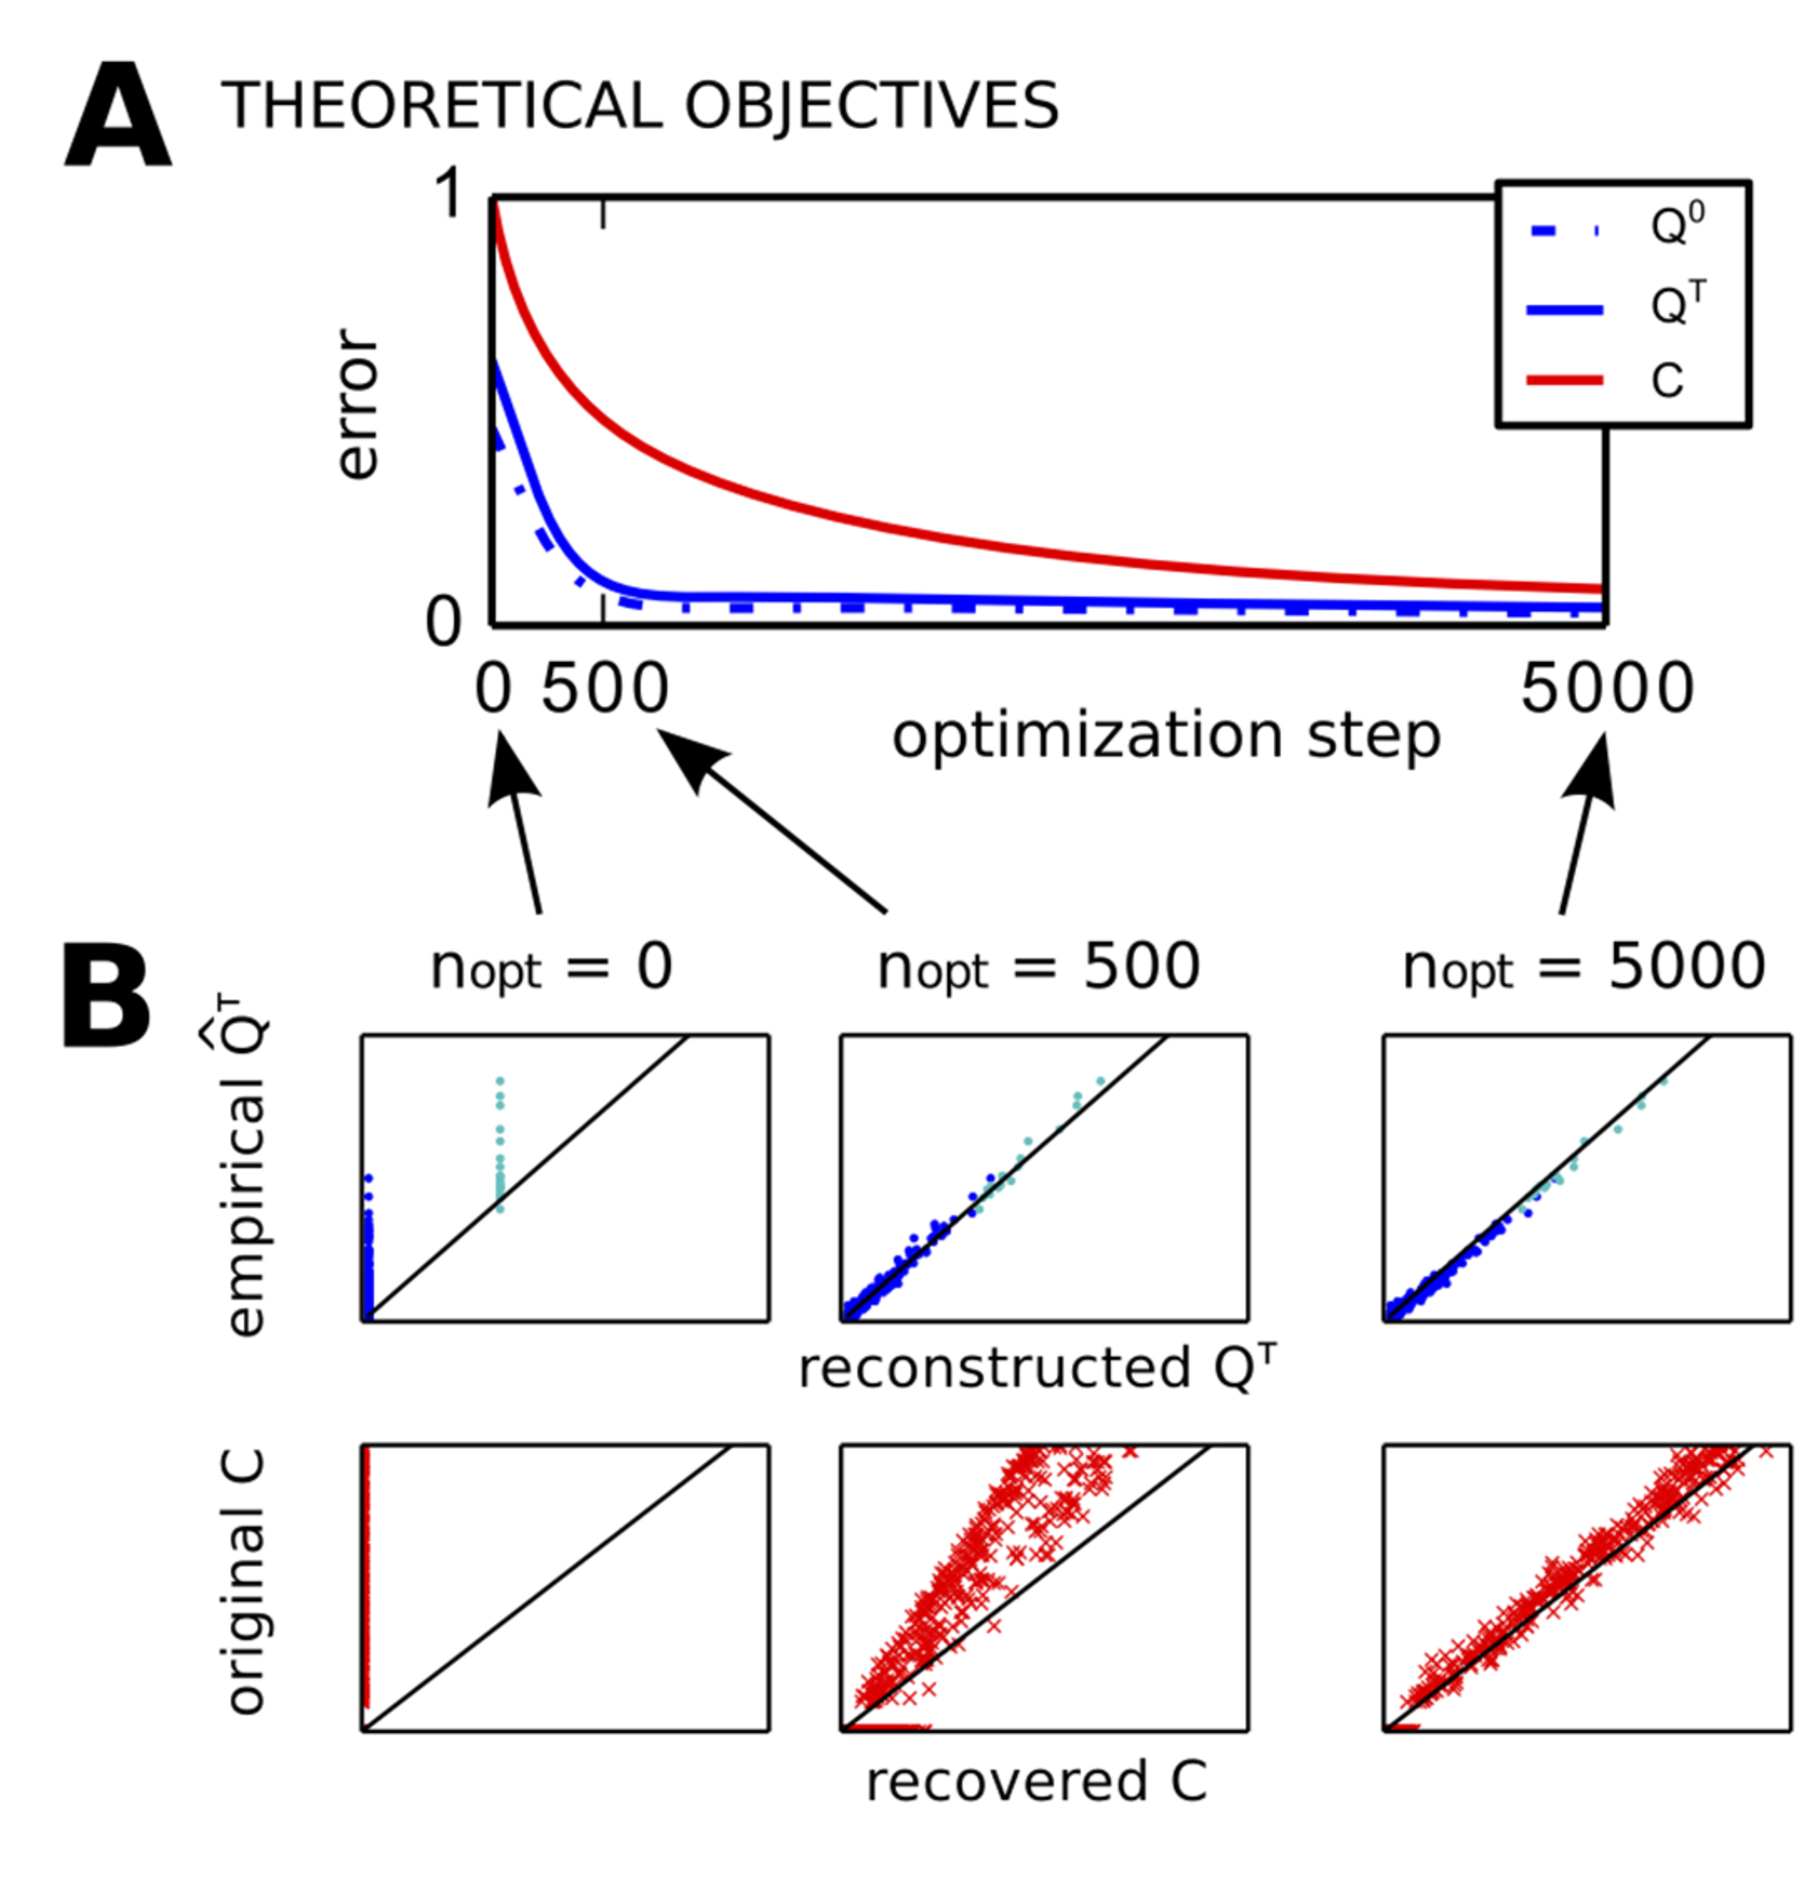
\includegraphics[width=0.8\columnwidth]{matt_fig.pdf}}
	\end{center}
\end{column}
\end{columns}
\end{frame}

\begin{frame}
\transdissolve
\frametitle{Bayesian estimation of parameters}
\begin{itemize}
		\pause
	\item Posterior probability of parameters $\rightarrow$ connectivity estimation 
		\pause
	\item Regularization $\rightarrow$ better estimation with few timepoints
		\pause
	\item Model comparison 
\end{itemize}
\end{frame}

\begin{frame}
\transdissolve
\frametitle{MAP estimate with uniform prior}
Singh et al. arXiv 2017
\pause
		\begin{equation*}
x(t')|x(t) \sim \mathcal{N}(x(t)expm(-\boldsymbol\lambda \Delta t), \mathbf{Q}^0-expm(-\boldsymbol\lambda \Delta t) 
\mathbf{Q}^0 expm(-\boldsymbol\lambda \Delta t)^T)\\[0.3cm]
 \pause
 \boldsymbol\lambda_{ij} = \delta_{ij} / \tau_i + C_{ij} \mathrm{;} \qquad \Delta t = t'-t\\[0.3cm]
 \pause
 x(t) \sim \mathcal{N}(0, \mathbf{Q}^0)\\[0.3cm]
 \pause
 P(X\mid\boldsymbol\lambda, \mathbf{Q}^0) = \prod_n^{N-1} P(x_{n+1}|x_n, \boldsymbol\lambda, \mathbf{Q}^0)P(x_n|\boldsymbol\lambda, \mathbf{Q}^0)\\[0.3cm]
 \pause
 P(\boldsymbol\lambda, \mathbf{Q}^0 | X) = \frac{P(X|\boldsymbol\lambda, \mathbf{Q}^0) P(\boldsymbol\lambda, \mathbf{Q}^0)}{P(X)}\\[0.3cm]
 \pause
 \boldsymbol\lambda^* = -logm(\sum_{n=1}^{N-1} x_{n+1}x_n^T (\sum_{n=1}^{N-1} x_n x_n^T)^{-1})/\Delta t \\[0.3cm]
 \pause
 C_{ij}^* = \boldsymbol\lambda_{ij}^* \qquad  \mathrm{for}\, i\ne j
		\end{equation*}
\end{frame}

%\begin{frame}
%\frametitle{MAP estimate for large scale networks}
%\begin{center}
%\includegraphics[width=0.7\columnwidth,valign=b]{}
%\end{center}
%\end{frame}

\begin{frame}
	\frametitle{Synthetic data}
	\begin{itemize}
		\item Simulated data from MOU 
		\item N=50 nodes
		\item Connection probability: 0.2
		\item Uniform distribution of weights
	\end{itemize}
\end{frame}
	
\begin{frame}
\frametitle{MAP estimate for small time samples}
\begin{center}
\only<1>{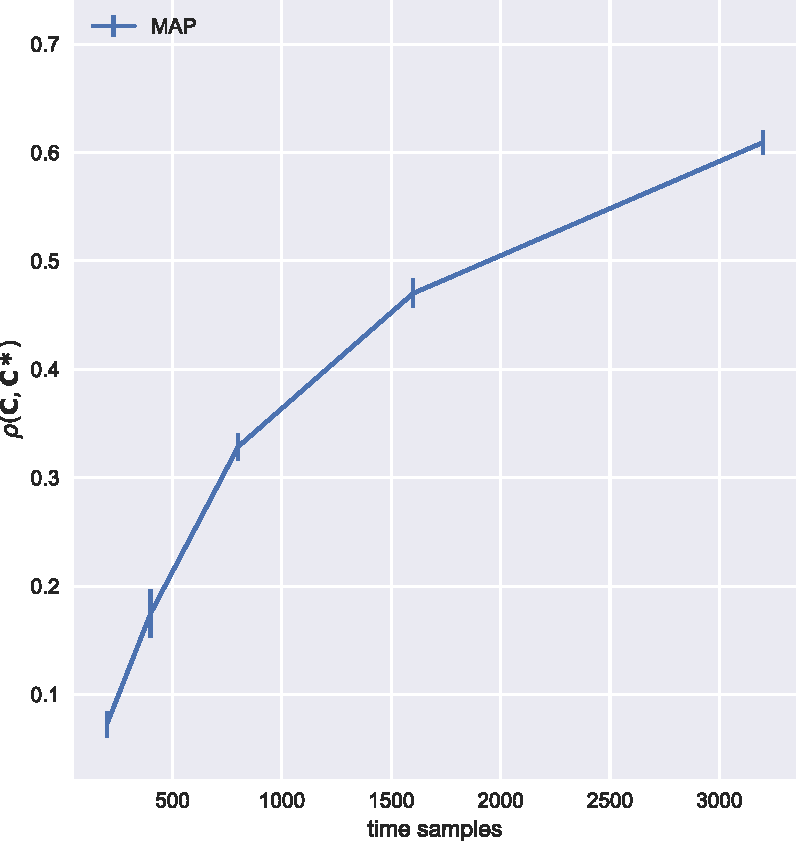
\includegraphics[width=0.65\columnwidth]{similarity_varyingT1}}
\only<2>{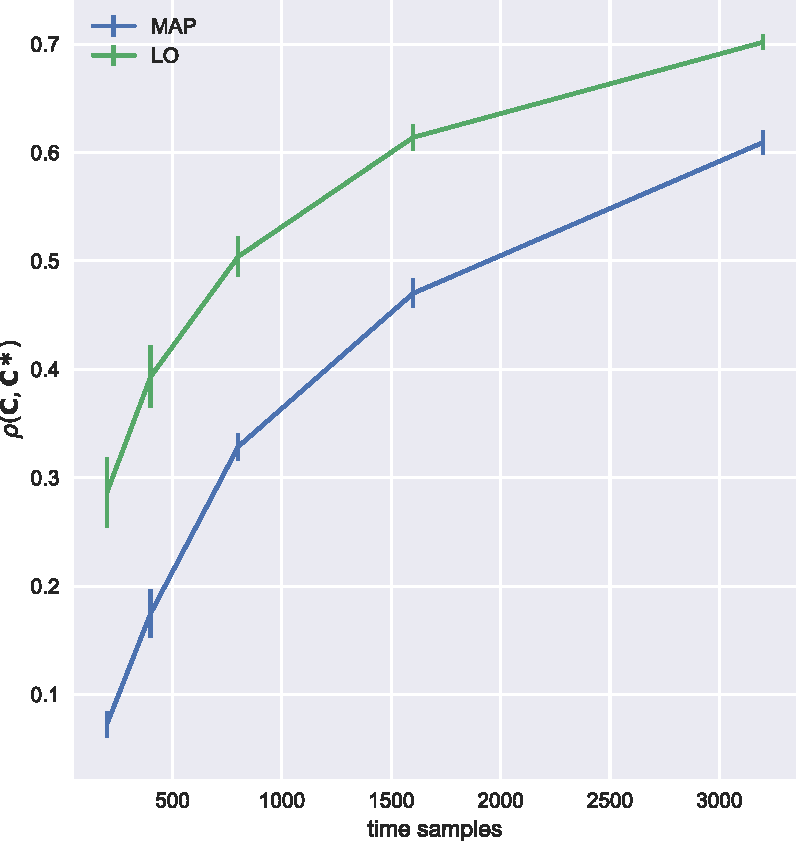
\includegraphics[width=0.65\columnwidth]{similarity_varyingT2}}
\end{center}
\end{frame}

\begin{frame}
\frametitle{Influence of weight values}
\begin{center}
\includegraphics[width=0.9\columnwidth]{similarity_varyingConnStren}
\end{center}
\end{frame}

\begin{frame}
\frametitle{True and predicted weights}
\begin{center}
	\includegraphics[width=0.99\columnwidth]{scatter_MAP_T1600}
\end{center}
\end{frame}

\begin{frame}
\frametitle{MAP estimate for small time samples}
\begin{center}
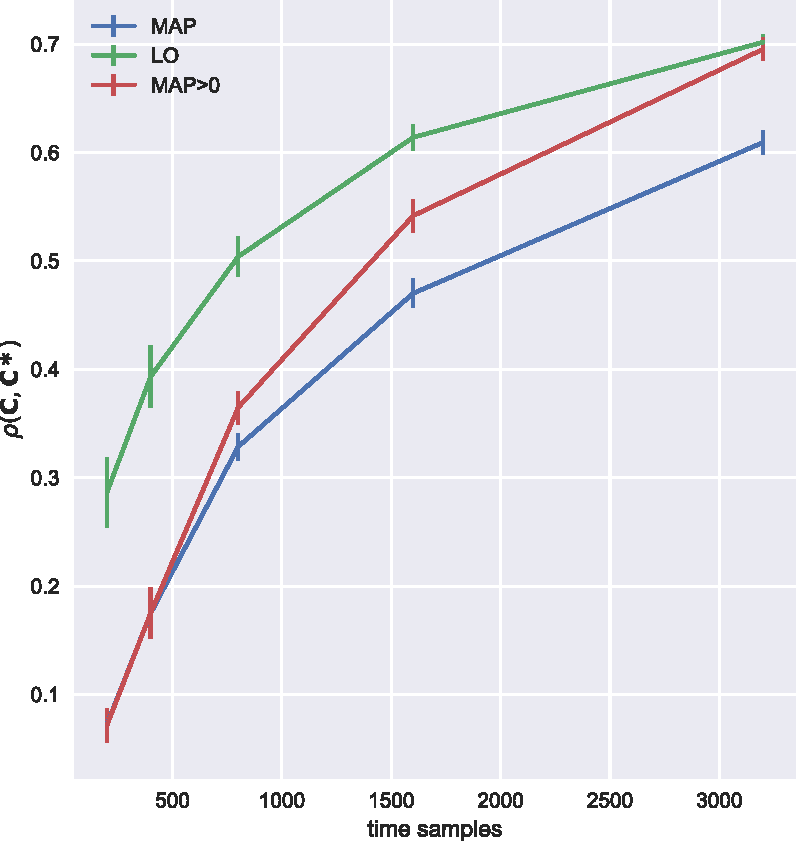
\includegraphics[width=0.65\columnwidth]{similarity_varyingT3}
\end{center}
\end{frame}

\begin{frame}
\frametitle{Next steps}
	\begin{itemize}
		\item Sparse network prior
		\item \ldots?
	\end{itemize}
\end{frame}

\begin{frame}
\frametitle{Acknowledgments}
\begin{columns}
\begin{column}{0.5\textwidth}
\begin{center}
	\alert<2>{Vicente Pallares}\\
\vspace{1cm}

\alert<2>{Matthieu Gilson}\\
\vspace{1cm}

\small Ana Sanjuan\\
\vspace{0.5cm}

\small Simone Kuhn\\
\vspace{0.5cm}

\small Dante Mantini\\
\vspace{0.5cm}

\small Gustavo Deco\\
\vspace{0.5cm}

\normalsize \alert<2>{John Cunningham}\\
\end{center}
\end{column}
\begin{column}{0.5\textwidth}
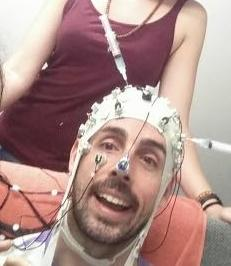
\includegraphics[width=0.5\columnwidth,valign=t]{vicente2}
\vspace{0.5cm}

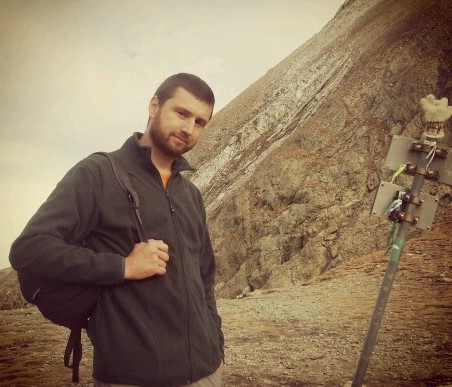
\includegraphics[width=0.5\columnwidth,valign=t]{matt}
\end{column}
\end{columns}
\end{frame}


\end{document}
